\documentclass[12pt]{report}
\renewcommand{\contentsname}{Table des matières}
\usepackage{polyglossia} %to set a language
\setmainlanguage{french}
\setotherlanguage{english}
\usepackage{hyperref}
\hypersetup{
	colorlinks=true,
	linkcolor=black,
	urlcolor=blue,
	citecolor=black,    
	pdftitle={},
	pdfauthor={Emmanuel ASSOHOU},
	pdfsubject={},
	pdfkeywords={},
}
\usepackage{xcolor} 
\usepackage{fontspec} %to specify a font
\usepackage{unicode-math} %to use all the math operators and symbols
\setmainfont{Times New Roman}
\setmathfont{Latin Modern Math}
\usepackage{enumitem} %to provide enhanced control over lists, allowing to customize the appearance and formatting of various types of lists
\usepackage{graphicx} %to use pictures in the document
\usepackage{setspace}
\setstretch{1.5}
\usepackage{tikzpagenodes} %provides convenient ways to work with page related coordinates and dimensions in TikZ
\usepackage[margin=2cm]{geometry}
\usepackage{ragged2e} %to provide enhanced justification commands for text alignment
\usepackage{amsmath} %ptovides advanced mathematical typesetting features and environments 
\usepackage{float}
\usepackage{emoji}
\usepackage{mfirstuc} %for capitalizing
\usepackage{stmaryrd}

\usepackage{tikz}
\usepackage{pgfplots}
\pgfplotsset{compat=1.15}
\pgfplotsset{soldot/.style={only marks,mark=*, line width=0.5pt, mark size=2pt}}
\pgfplotsset{holdot/.style={fill=white,only marks,mark=*, line width=1pt, mark size=2pt}}
\renewcommand{\contentsname}{Table des matières}
\usepackage{polyglossia} %to set a language
\setmainlanguage{french}
\setotherlanguage{english}
\usepackage{hyperref}
\hypersetup{
	colorlinks=true,
	linkcolor=black,
	urlcolor=blue,
	citecolor=black,    
	pdftitle={},
	pdfauthor={Emmanuel ASSOHOU},
	pdfsubject={},
	pdfkeywords={},
}
\usepackage{xcolor} 
\usepackage{amsmath}
\usepackage{longtable}
\usepackage{listings} % Include the listings package

\begin{document}
Les données ci-dessous, obtenues sur le site de la BECEAO serviront de base de travail pour notre projet éconmétrique.
	% Table generated by Excel2LaTeX from sheet 'Feuil1'
\input{tables/table-1}


Grâce à ces données nous avons pu tracer les nuages de points entre les rubriques \guillemetleft alimentation \guillemetright et \guillemetleft Boissons alcolisées, Tabac et stupéfiants \guillemetright. L'alimentation représentera la variable $x$ et les Boissons alcolisées, Tabac et stupéfiants, la varible $y$.

\begin{figure}[htbp]
	\centering
	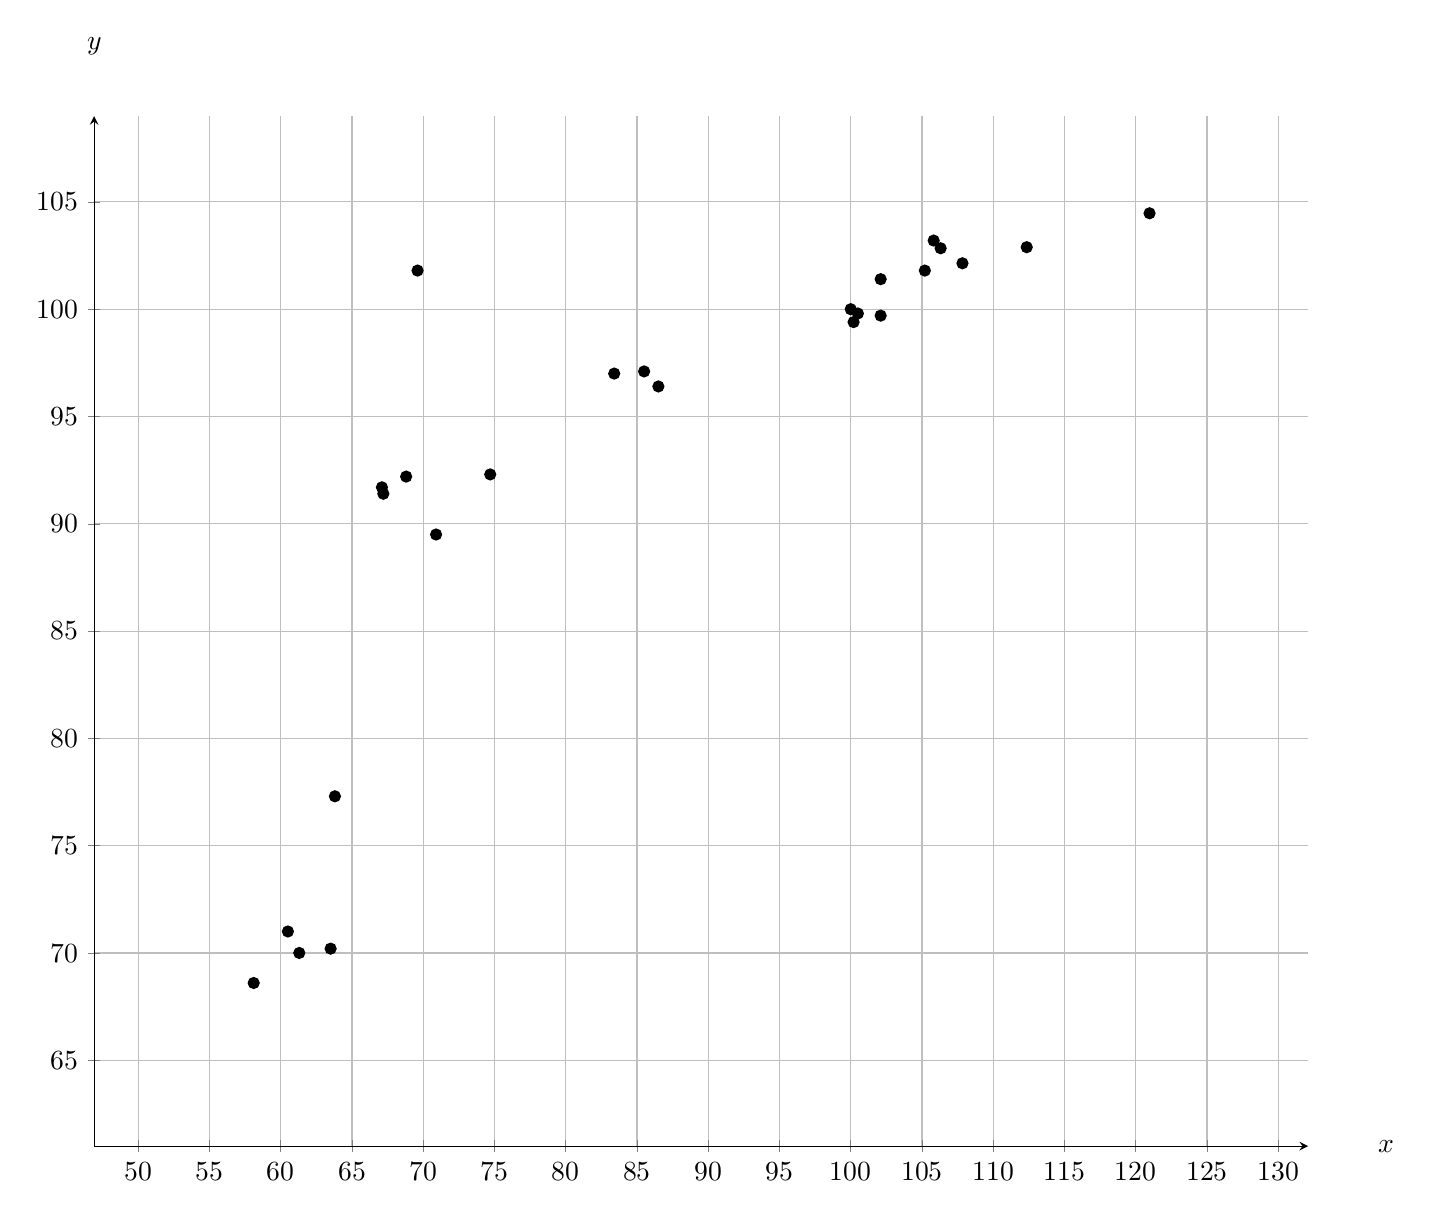
\begin{tikzpicture}
		\begin{axis}[
			xlabel={$x$},
			ylabel={$y$},
			legend pos=north east,
			grid=major,
			xmin=54, xmax=125,
			ymin=65, ymax=105,
			axis x line=middle, 
			axis y line=middle, 
			samples=1000, 
			xlabel = $x$, 
			ylabel=$y$,
			enlargelimits,
			xlabel style={at={(ticklabel* cs:1.05)}, anchor=west}, % Place le nom de l'axe x à droite de l'axe
			ylabel style={at={(ticklabel* cs:1.05)}, anchor=south}, % Place le nom de l'axe y au-dessus de l'axe
			width=17cm,
			]
			
			\addplot[mark=*, only marks] coordinates {
				(58.1,68.6)
				(63.5,70.2)
				(61.3,70)
				(60.5,71)
				(63.8,77.3)
				(67.1,91.7)
				(69.6,101.8)
				(67.2,91.4)
				(68.8,92.2)
				(70.9,89.5)
				(74.7,92.3)
				(83.4,97)
				(85.5,97.1)
				(86.5,96.4)
				(100.5,99.8)
				(100.2,99.4)
				(102.1,99.7)
				(100,100)
				(102.1,101.4)
				(105.2,101.8)
				(105.82,103.2)
				(106.31,102.84)
				(107.84,102.14)
				(112.35,102.89)
				(120.97,104.47)
				
			};
			
			%\addplot[domain=50:130, line width=0.95pt]{0.3473297*x+ 7.89647} node[pos=0.95, anchor=east]{$\text{1.116545}x+\text{1.258177}$};
			
		\end{axis}
	\end{tikzpicture}
\end{figure}
\end{document}